\documentclass[border=0.5pt]{standalone}
\usepackage{tikz}
\usetikzlibrary{calc}

\renewcommand{\familydefault}{\sfdefault}
\begin{document}
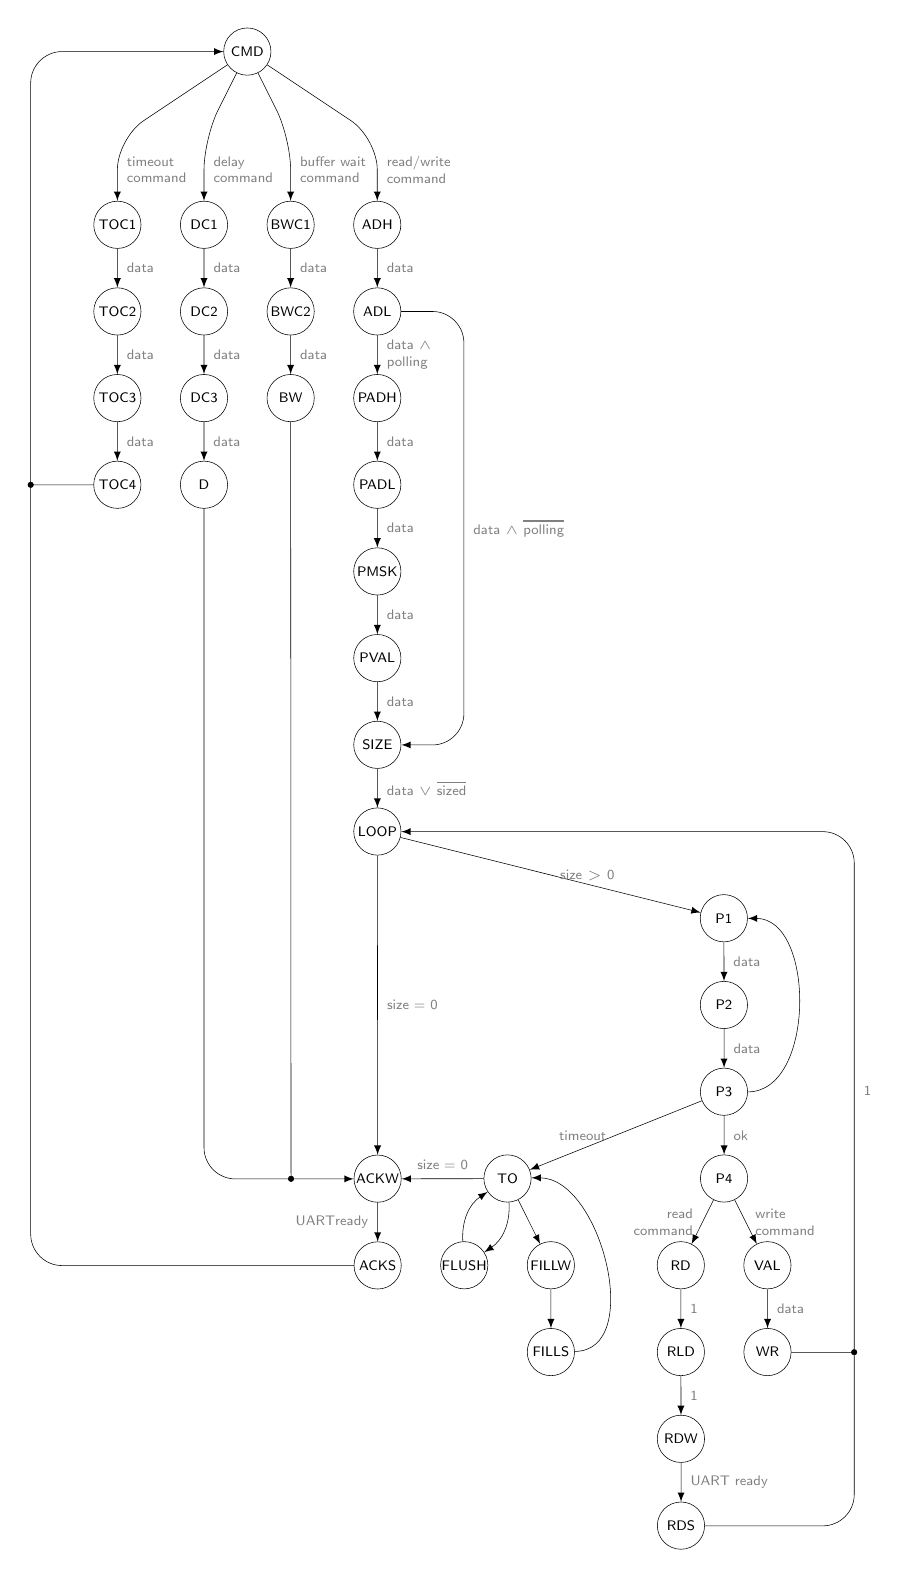
\begin{tikzpicture}[scale=1.1,
	state/.style={draw,circle,minimum width=0.6cm, font=\tiny, inner sep=0, very thin},
	bullet/.style={circle,draw,fill=black,minimum width=2, inner sep=0},
	cond/.style={gray,font=\tiny,midway},
	redge/.style={rounded corners=0.4cm}]
	\tikzset{every path/.style={line width=0.2pt}}
	\tikzset{>=latex}
	\node [state] (cmd) at (0,0) {CMD};
	\node [state] (adh) at ($(cmd) + (1.5,-2)$) {ADH};
	\node [state] (adl) at ($(adh) + (0,-1)$) {ADL};
	\node [state] (padh) at ($(adl) + (0,-1)$) {PADH};
	\node [state] (padl) at ($(padh) + (0,-1)$) {PADL};
	\node [state] (pmsk) at ($(padl) + (0,-1)$) {PMSK};
	\node [state] (pval) at ($(pmsk) + (0,-1)$) {PVAL};
	\node [state] (size) at ($(pval) + (0,-1)$) {SIZE};
	\node [state] (loop) at ($(size) + (0,-1)$) {LOOP};
	\node [state] (p1) at ($(loop) + (4,-1)$) {P1};
	\node [state] (p2) at ($(p1) + (0,-1)$) {P2};
	\node [state] (p3) at ($(p2) + (0,-1)$) {P3};
	\node [state] (p4) at ($(p3) + (0,-1)$) {P4};
	\node [state] (rd) at ($(p4) + (-0.5,-1)$) {RD};
	\node [state] (rld) at ($(rd) + (0,-1)$) {RLD};
	\node [state] (rdw) at ($(rld) + (0,-1)$) {RDW};
	\node [state] (rds) at ($(rdw) + (0,-1)$) {RDS};
	\node [state] (val) at ($(p4) + (0.5,-1)$) {VAL};
	\node [state] (wr) at ($(val) + (0,-1)$) {WR};
	\node [state] (to) at ($(p3) + (-2.5,-1)$) {TO};
	\node [state] (fillw) at ($(to) + (0.5,-1)$) {FILLW};
	\node [state] (fills) at ($(fillw) + (0,-1)$) {FILLS};
	\node [state] (flush) at ($(to) + (-0.5,-1)$) {FLUSH};
	\node [state] (ackw) at ($(to) + (-1.5,0)$) {ACKW};
	\node [state] (acks) at ($(ackw) + (0,-1)$) {ACKS};
	\node [state] (bwc1) at ($(cmd) + (0.5,-2)$) {BWC1};
	\node [state] (bwc2) at ($(bwc1) + (0,-1)$) {BWC2};
	\node [state] (bw) at ($(bwc2) + (0,-1)$) {BW};
	\node [state] (dc1) at ($(cmd) + (-0.5,-2)$) {DC1};
	\node [state] (dc2) at ($(dc1) + (0,-1)$) {DC2};
	\node [state] (dc3) at ($(dc2) + (0,-1)$) {DC3};
	\node [state] (d) at ($(dc3) + (0,-1)$) {D};
	\node [state] (toc1) at ($(cmd) + (-1.5,-2)$) {TOC1};
	\node [state] (toc2) at ($(toc1) + (0,-1)$) {TOC2};
	\node [state] (toc3) at ($(toc2) + (0,-1)$) {TOC3};
	\node [state] (toc4) at ($(toc3) + (0,-1)$) {TOC4};
	
	\node (dot1) [bullet] at ($(wr)+(1,0)$) {};
	\node (dot2) [bullet] at ($(ackw)+(-1,0)$) {};
	\node (dot3) [bullet] at ($(toc4)+(-1,0)$) {};
	
	\draw [->, redge] (cmd) -- ($(adh)+(0,1)$) -- (adh) node [cond, right, align=left] {read/write \\ command};
	\draw [->, redge] (cmd) -- ($(bwc1)+(0,1)$) -- (bwc1) node [cond, right, align=left] {buffer wait \\ command};
	\draw [->, redge] (cmd) -- ($(dc1)+(0,1)$) -- (dc1) node [cond, right, align=left] {delay \\ command};
	\draw [->, redge] (cmd) -- ($(toc1)+(0,1)$) -- (toc1) node [cond, right, align=left] {timeout \\ command};
	\draw [->] (adh) -- (adl) node [cond, right, align=left] {data};
	\draw [->, redge] (adl) -- ++(1,0) |- (size) node [cond, right, near start] {data $\land$ $\overline{\mbox{polling}}$};
	\draw [->] (adl) -- (padh) node [cond, right, align=left] {data $\land$ \\ polling};
	\draw [->] (padh) -- (padl) node [cond, right] {data};
	\draw [->] (padl) -- (pmsk) node [cond, right] {data};
	\draw [->] (pmsk) -- (pval) node [cond, right] {data};
	\draw [->] (pval) -- (size) node [cond, right] {data};
	\draw [->] (size) -- (loop) node [cond, right] {data $\lor$ $\overline{\mbox{sized}}$};
	\draw [->] (loop) -- (p1) node [cond, right] {size $>$ 0};
	\draw [->] (p1) -> (p2) node [cond, right] {data};
	\draw [->] (p2) -> (p3) node [cond, right] {data};
	\draw [->] (p3) -> (p4) node [cond, right] {ok};
	\draw [->] (p3) edge [bend right=90] (p1);
	\draw [->] (p4) -> (rd) node [cond, left, align=right] {read \\ command};
	\draw [->] (p4) -> (val) node [cond, right, align=left] {write \\ command};
	\draw [->] (rd) -> (rld) node [cond, right] {1};
	\draw [->] (rld) -> (rdw) node [cond, right] {1};
	\draw [->] (rdw) -> (rds) node [cond, right] {UART ready};
	\draw [->] (val) -> (wr) node [cond, right] {data};
	\draw [->, redge] (wr) -- (dot1) |- (loop) node [cond, right, near start] {1};
	\draw [redge] (rds) -| (dot1);
	\draw [->] (p3) -- (to) node [cond, left] {timeout};
	\draw [->] (to) -- (fillw);
	\draw [->] (fillw) -- (fills);
	\draw [->] (fills.e) to [out=0, in=0] (to.e);
	\draw [->] (to) edge [bend left] (flush);
	\draw [->] (flush) edge [bend left] (to);
	\draw [->] (to) -- (ackw) node [cond, above] {size = 0};
	\draw [->] (ackw) -- (acks) node [cond, left] {UART \\ ready};
	\draw [->] (loop) -- (ackw) node [cond, right, align=left] {size = 0};
	\draw [->] (bwc1) -- (bwc2) node [cond, right] {data};
	\draw [->] (bwc2) -- (bw) node [cond, right] {data};
	\draw [->] (bw) -- (dot2) -- (ackw);
	\draw [->] (dc1) -- (dc2) node [cond, right] {data};
	\draw [->] (dc2) -- (dc3) node [cond, right] {data};
	\draw [->] (dc3) -- (d) node [cond, right] {data};
	\draw [->] (toc1) -- (toc2) node [cond, right] {data};
	\draw [->] (toc2) -- (toc3) node [cond, right] {data};
	\draw [->] (toc3) -- (toc4) node [cond, right] {data};
	\draw [redge] (d) |- (dot2);
	\draw (toc4) -- (dot3);
	\draw [redge] (acks) -| (dot3);
	\draw [->, redge] (dot3) |- (cmd);
\end{tikzpicture}
\end{document}
